% !TEX TS-program = pdflatex
% !TEX encoding = UTF-8 Unicode

% This is a simple template for a LaTeX document using the "article" class.
% See "book", "report", "letter" for other types of document.

\documentclass[11pt]{article} % use larger type; default would be 10pt

\usepackage[utf8]{inputenc} % set input encoding (not needed with XeLaTeX)

%%% Examples of Article customizations
% These packages are optional, depending whether you want the features they provide.
% See the LaTeX Companion or other references for full information.

%%% PAGE DIMENSIONS
\usepackage{geometry} % to change the page dimensions
\geometry{a4paper} % or letterpaper (US) or a5paper or....
% \geometry{margin=2in} % for example, change the margins to 2 inches all round
% \geometry{landscape} % set up the page for landscape
%   read geometry.pdf for detailed page layout information

\usepackage{graphicx} % support the \includegraphics command and options

% \usepackage[parfill]{parskip} % Activate to begin paragraphs with an empty line rather than an indent

%%% PACKAGES
\usepackage{booktabs} % for much better looking tables
\usepackage{array} % for better arrays (eg matrices) in maths
\usepackage{paralist} % very flexible & customisable lists (eg. enumerate/itemize, etc.)
\usepackage{verbatim} % adds environment for commenting out blocks of text & for better verbatim
\usepackage{subfig} % make it possible to include more than one captioned figure/table in a single float
% These packages are all incorporated in the memoir class to one degree or another...

%%% HEADERS & FOOTERS
\usepackage{fancyhdr} % This should be set AFTER setting up the page geometry
\pagestyle{fancy} % options: empty , plain , fancy
\renewcommand{\headrulewidth}{0pt} % customise the layout...
\lhead{}\chead{}\rhead{}
\lfoot{}\cfoot{\thepage}\rfoot{}

%%% SECTION TITLE APPEARANCE
\usepackage{sectsty}
\allsectionsfont{\sffamily\mdseries\upshape} % (See the fntguide.pdf for font help)
% (This matches ConTeXt defaults)

%%% ToC (table of contents) APPEARANCE
\usepackage[nottoc,notlof,notlot]{tocbibind} % Put the bibliography in the ToC
\usepackage[titles,subfigure]{tocloft} % Alter the style of the Table of Contents
\usepackage{hyperref}
\usepackage{xparse}
\usepackage{amsmath}


\hypersetup{
    colorlinks=true,
    linkcolor=blue,
    filecolor=magenta,      
    urlcolor=cyan,
}

\renewcommand{\cftsecfont}{\rmfamily\mdseries\upshape}
\renewcommand{\cftsecpagefont}{\rmfamily\mdseries\upshape} % No bold!

%%% END Article customizations

%%% The "real" document content comes below...

\title{Assignment 1}
\author{Ronghao Yang ID:20511820\\Session: CS698, 4:00pm-5:20pm}
%\date{} % Activate to display a given date or no date (if empty),
         % otherwise the current date is printed 
         
\graphicspath{ {graphs/} }

\begin{document}
\maketitle

\section{Exercise 1}

\subsection{question 1}
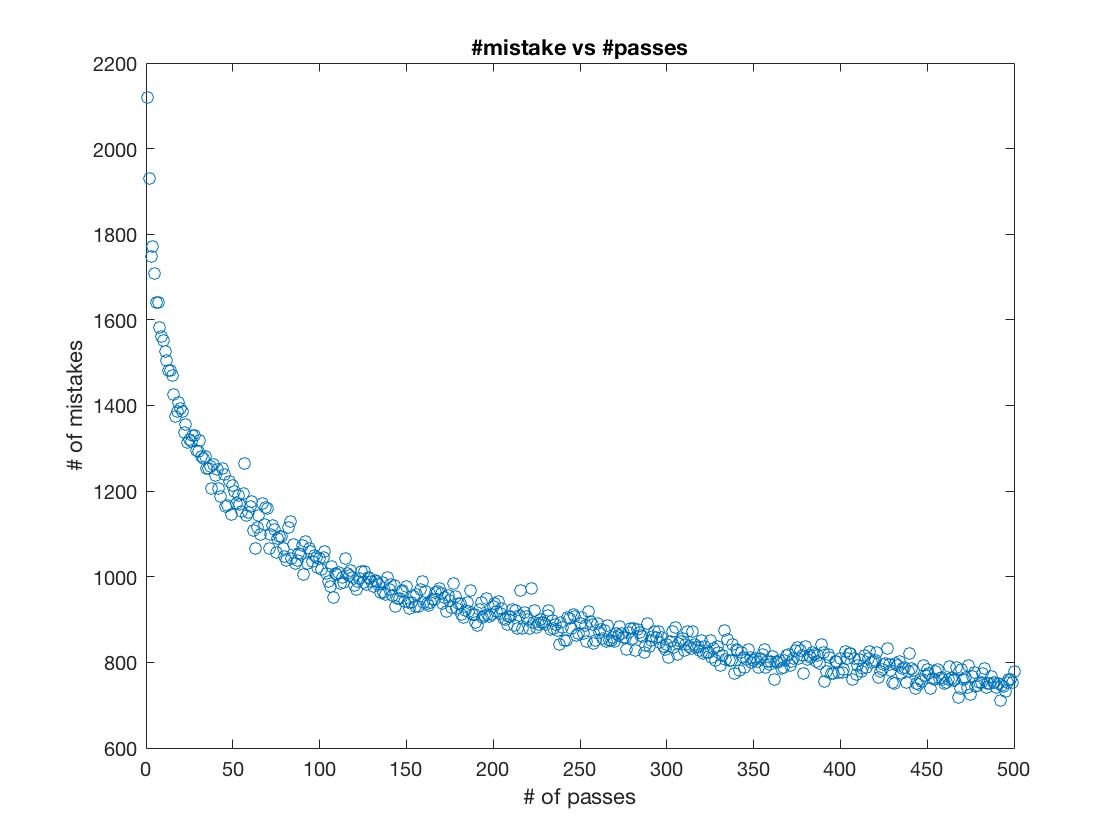
\includegraphics[scale=0.4]{e1q1.jpg}
\subsection{question 2}
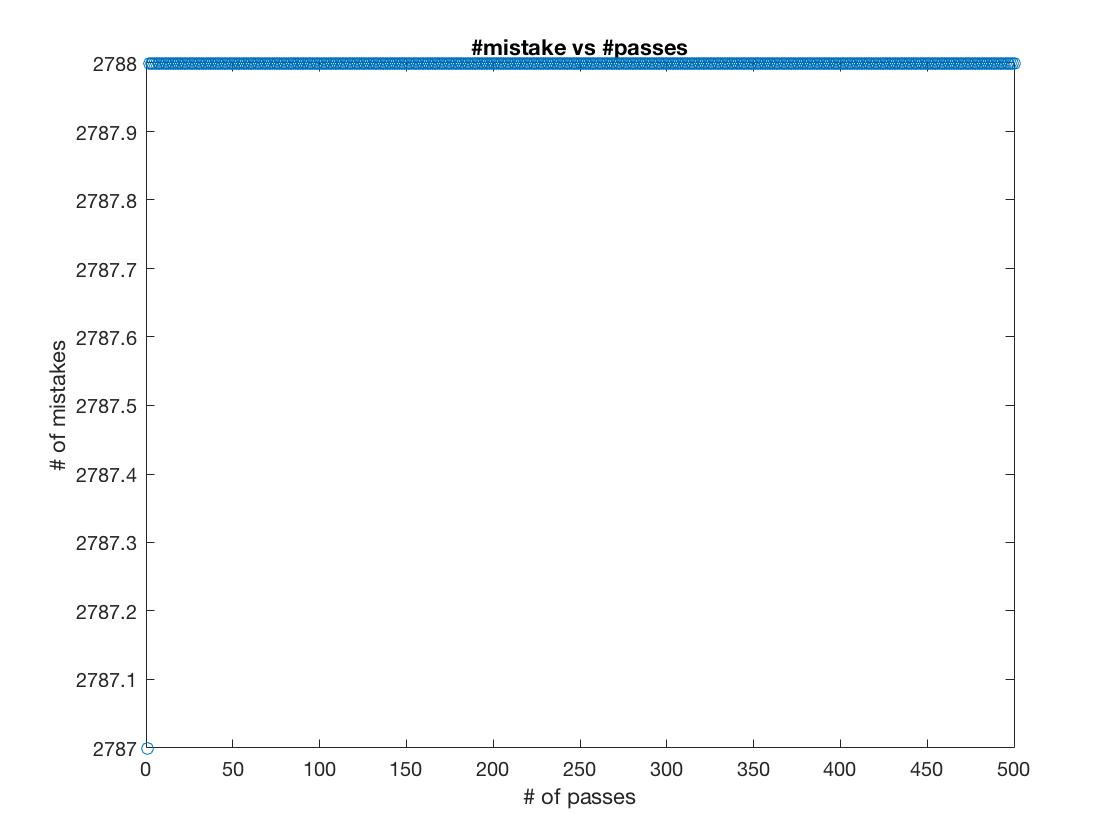
\includegraphics[scale=0.4]{e1q2.jpg}
\subsection{question 3}
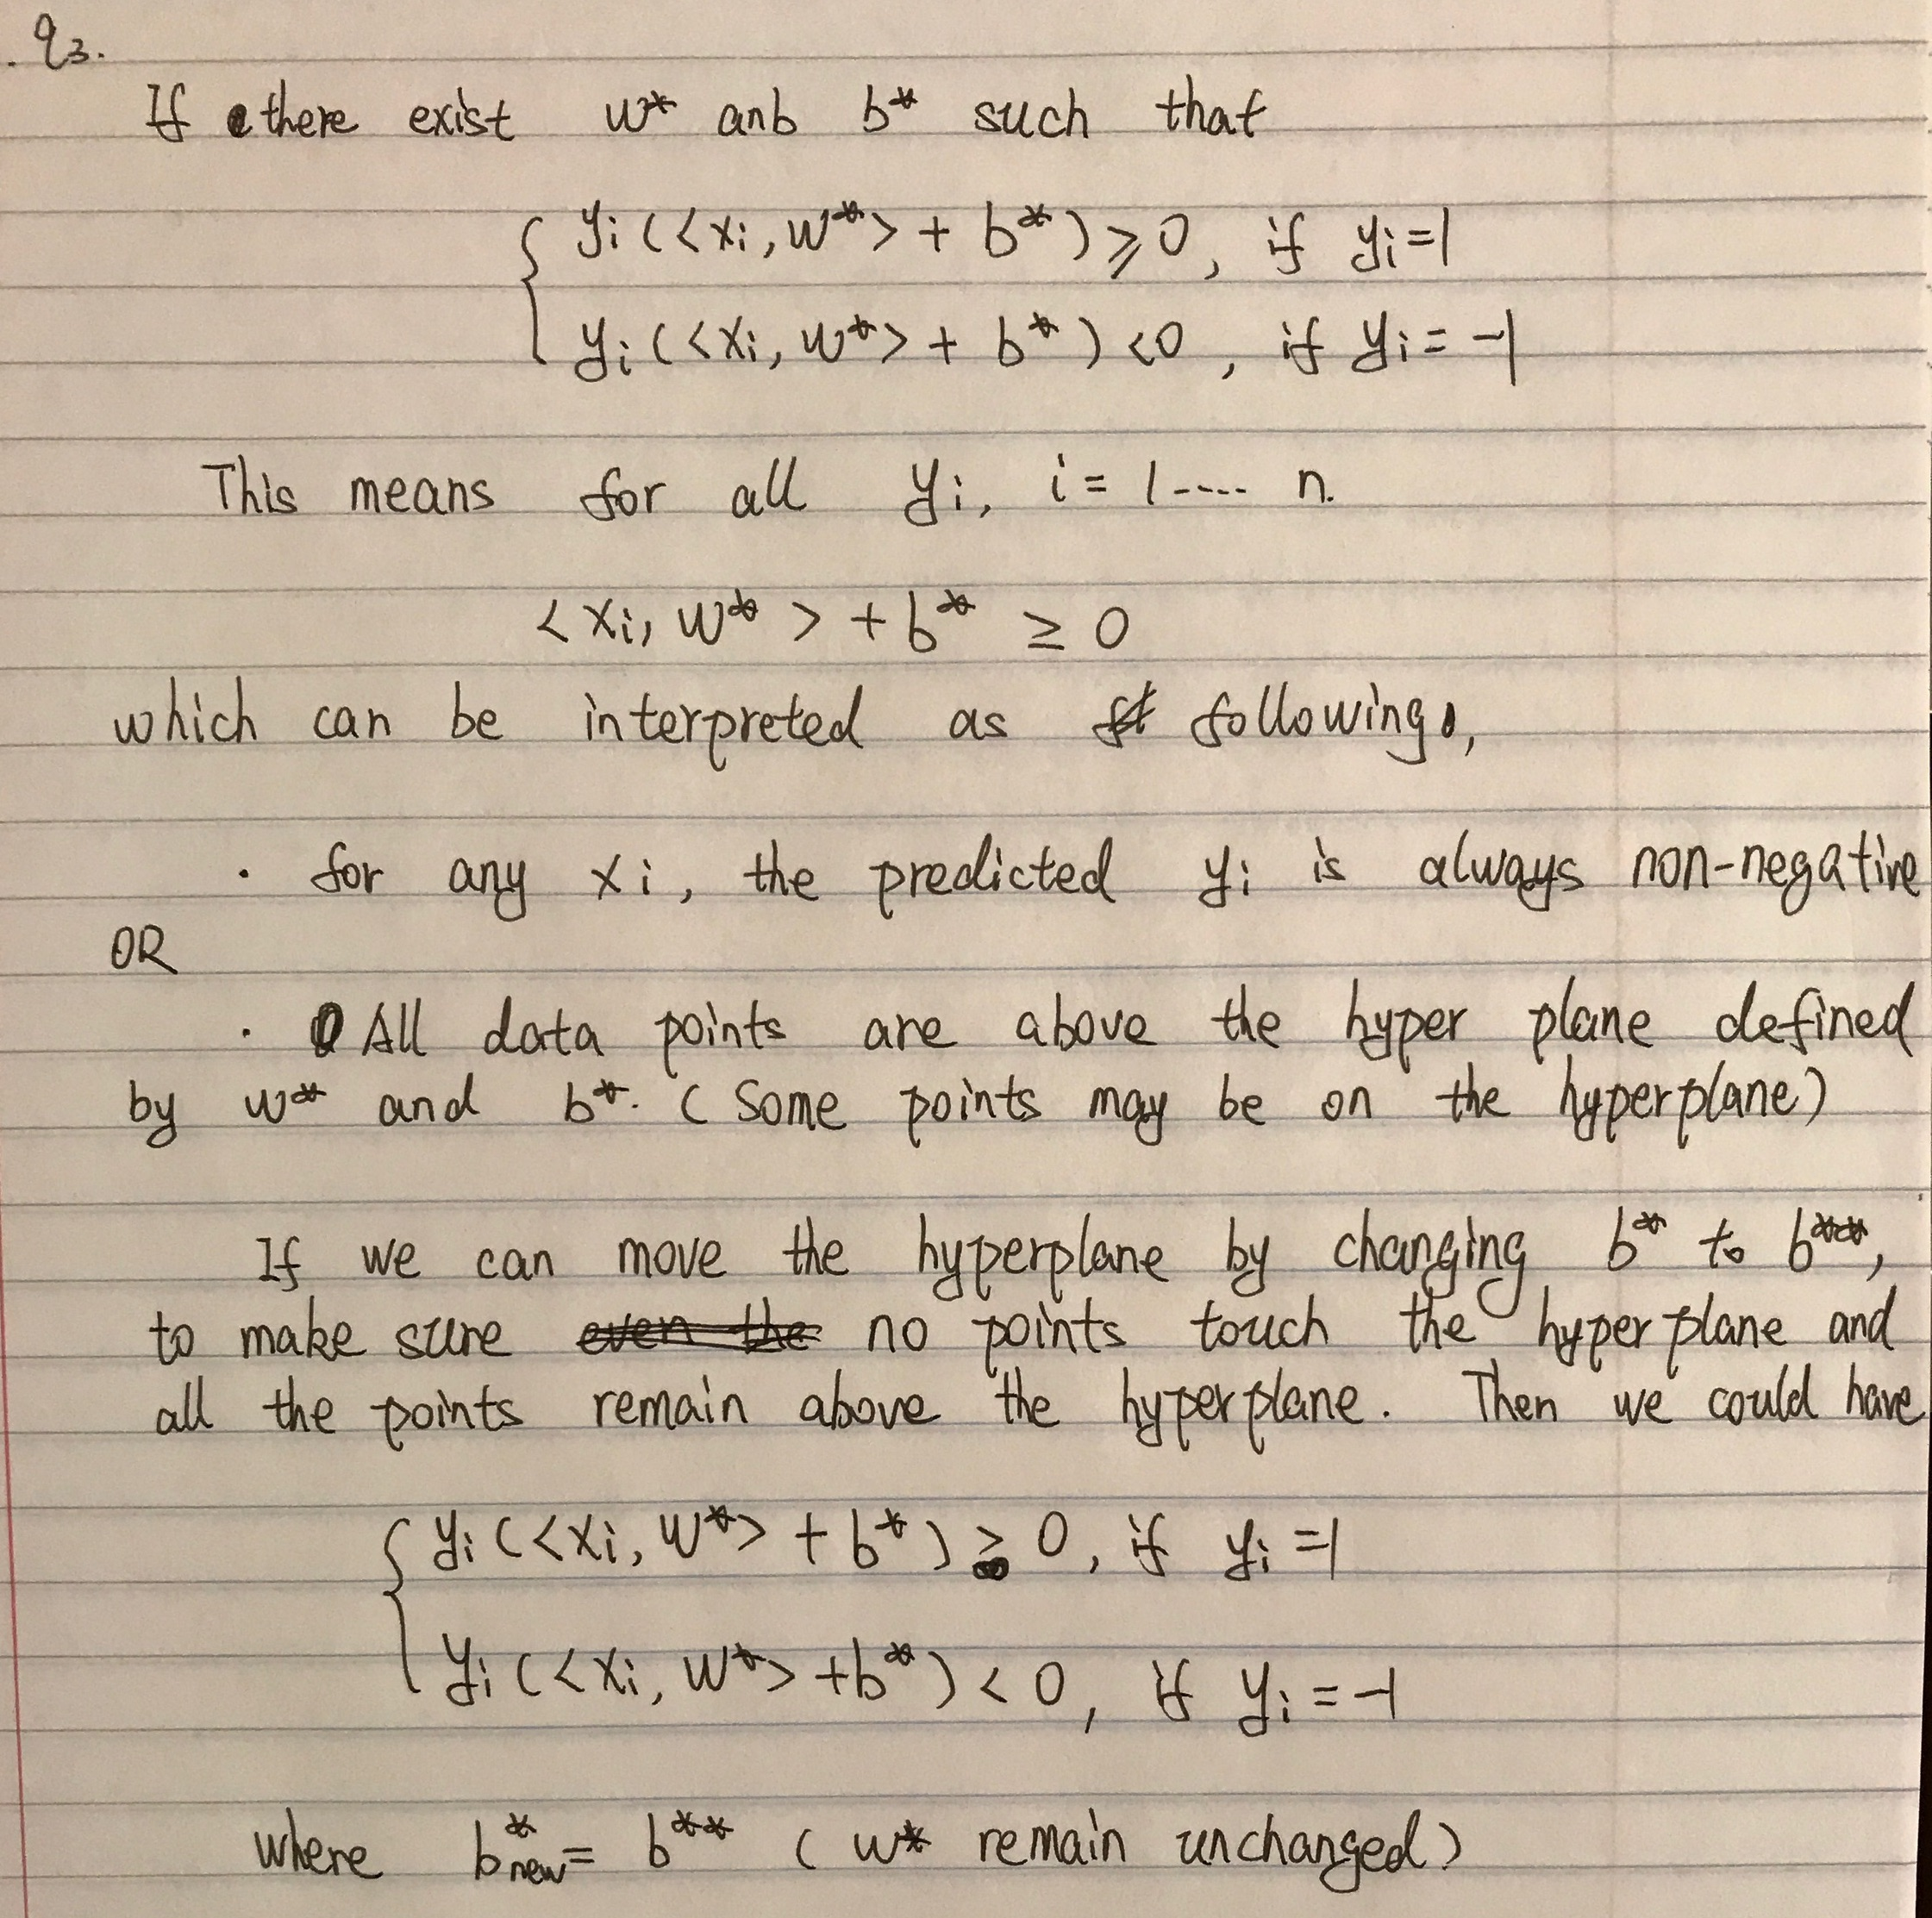
\includegraphics[scale=0.2]{e1q3.jpeg}
\subsection{question 4}
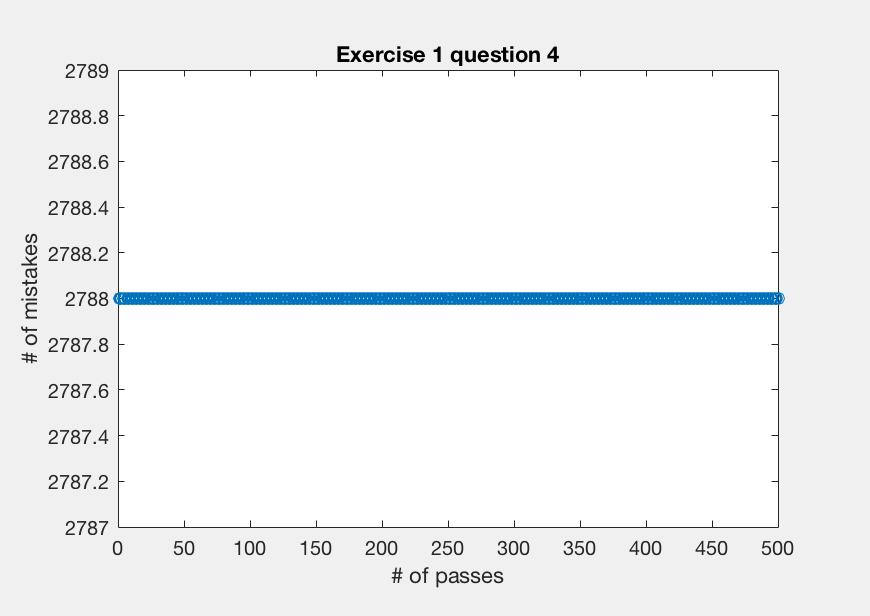
\includegraphics[scale=1]{e1q4}
StepSize: \\
As \href{https://piazza.com/class/j6y0higvsx37d0?cid=26}{what has been discussed} on Piazza, both $W$ and $b$ are always positive, since all the values in X are also possitive, $<W,X>+b$ is always evaluated to positive. This means, whenever $y_{i}$ is -1, $y_{i}(<x_{i}, w^{*}> + b^{*})$ is negative, which is reported as a mistake. Therefore, the total number of mistake in each pass is always the number of $-1$s in y. Tuning the step\_size wouldn't reduce the number of mistakes made by the algorithm. [please refer to question 5 for calculating step size using cross validation]
\subsection{question 5}
To transform the data matrix $X$ so that the non-negativity assumption can be ignored, we do the following: \\
$X_{new} = [X\,\,{-X}]$, eq: if $X = [x_{1};\,x_{2};....\,;x_{n}]$, then $X_{new} = [x_{1}\,\,{-x_{1}}; \,x_{2}\,\,{-x_{2}};....\,;x_{n}\,\,{-x_{n}}]$\\ 
Regarding the data set we have, the original data set has dimension $4601\times57$, after transformation, $X_{new}$ has dimension $4601\times114$. If we append ones to X[then w is (w;b)] before we do the transformation, our new data matrix has dimension $4601\times116$.\\
By doing so, the prediction can still be negative even no negative numbers show in the weight vector w. We know that w = \{max(w,0)$-$ max(-w,0)\}
\begin{equation}
Y_{predictions} = <x,max(w,0)> + <-x,max(-w,0)>
\end{equation}
The new weight vector w in the winnow algorithms is (max(w,0),max(w,0)).\\
By running cross validation (step size from $\dfrac{1}{m}$ to $\dfrac{10}{m}$, where m is the maximum value in X) on the new transformed matrix, the optimal is found to be $\dfrac{2}{m}$.\\
Using the optimal step size, the graph is the following:\\
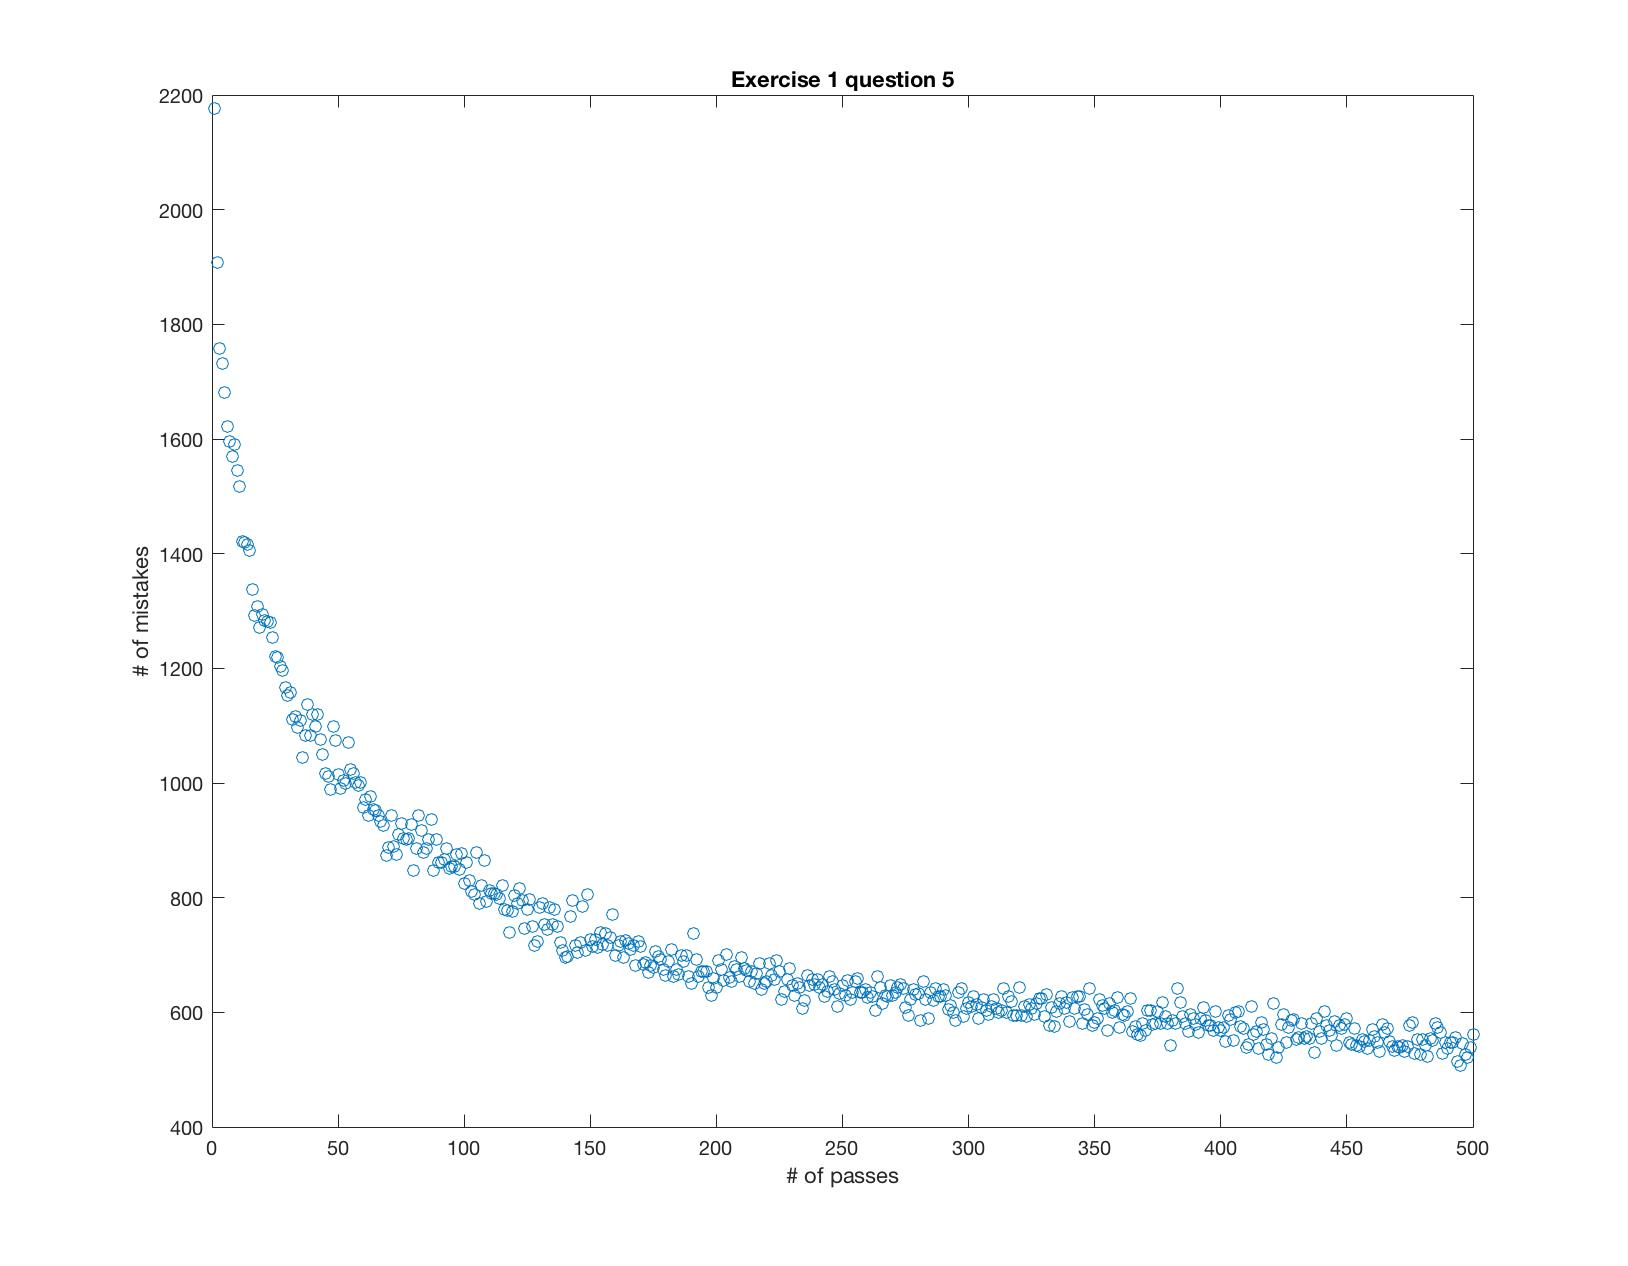
\includegraphics[scale=0.3]{e1q5.jpg}

\subsection{question 6}
Perceptron algorithm uses additive update, while Winnow algorithm uses multiplicative update. Both algorithms are computationally efficient, and guaranteed to find a hyperplane for linearly separable data. However, perceptron algorithm run in $O(n)$ time, winnow algorithm runs in $O(logn)$ time, where n is the number of features. After adding $1000$ random features to the data set, we can see that winnow algorithm converges faster than perceptron algorithm. When a data set has a large number of features, winnow algorithm is preferred.\\
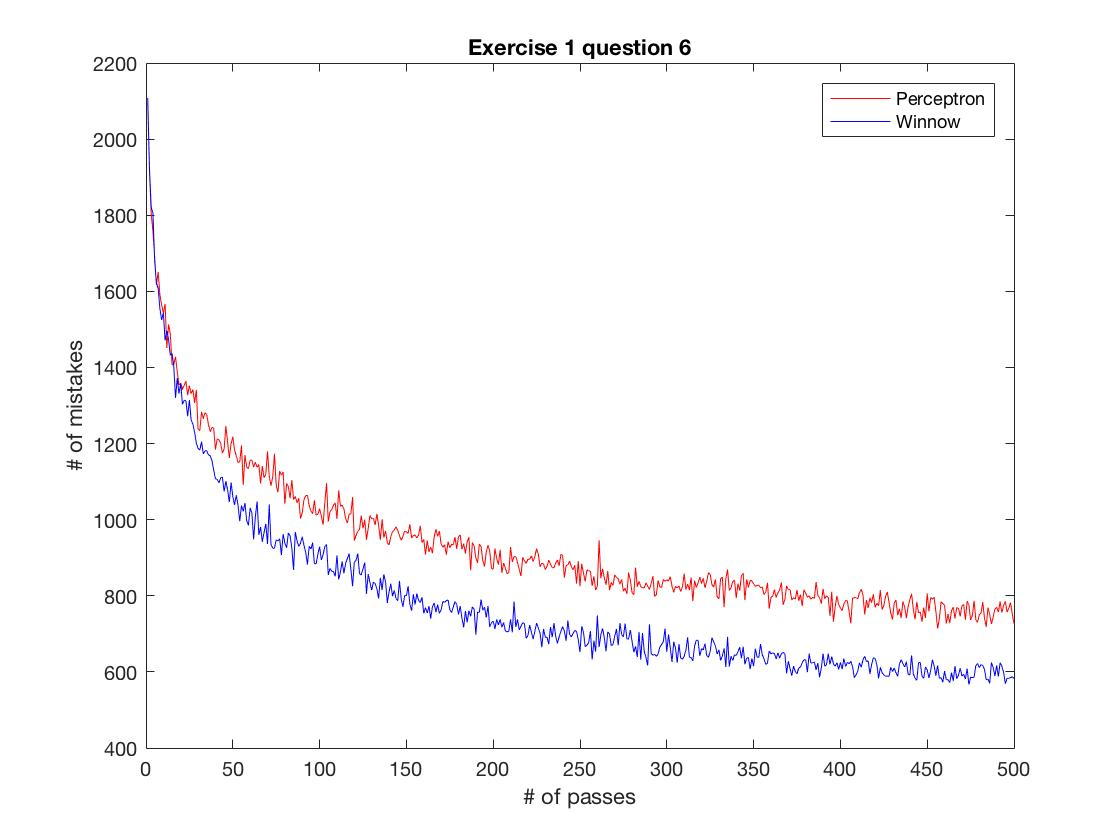
\includegraphics[scale=0.4]{e1q6.jpg}
\section{Exercise 2}
\subsection{question 1}
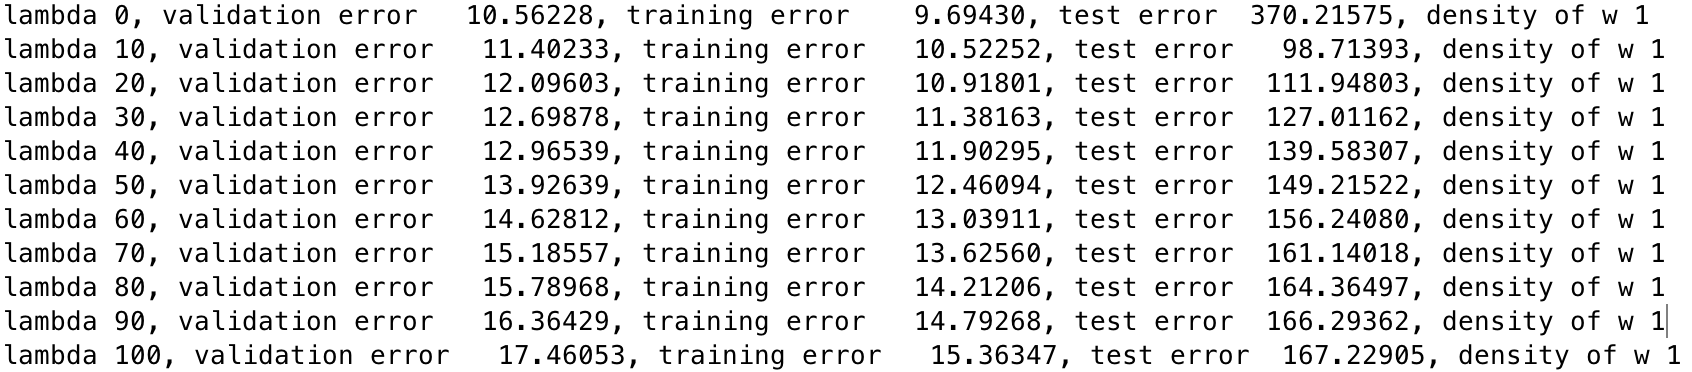
\includegraphics[scale=0.5]{e2q1}\\
\subsection{question 2}
1. Multiplying $y$ by $10^{6}$\\\\
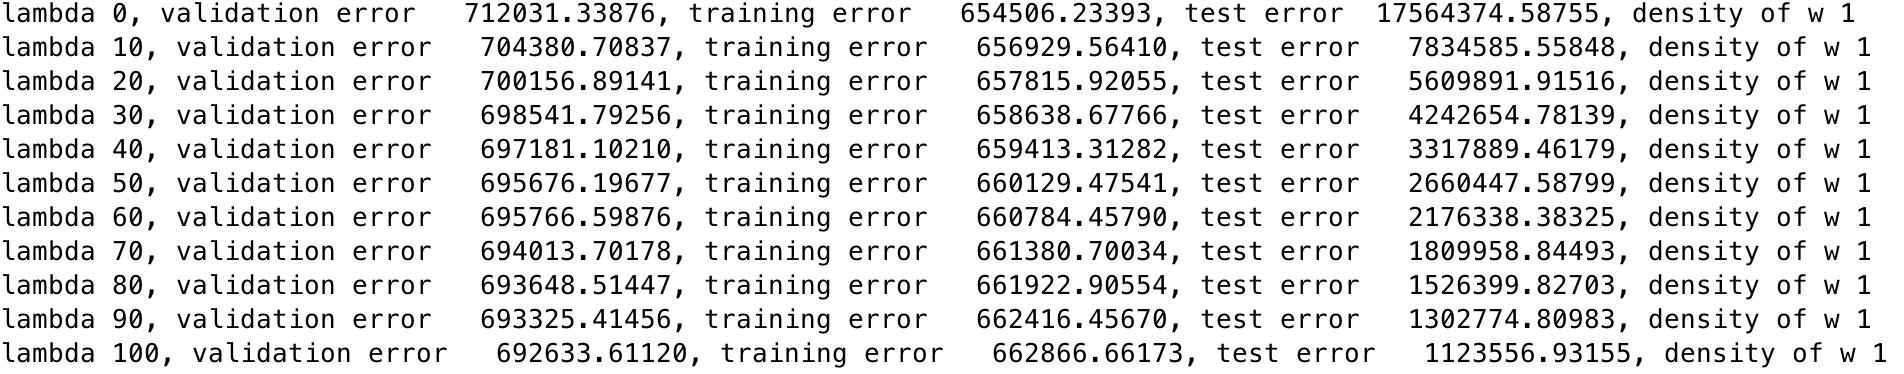
\includegraphics[scale=0.5]{e2q2y}\\
2. Multiplying $x$ by $10^{3}$\\\\
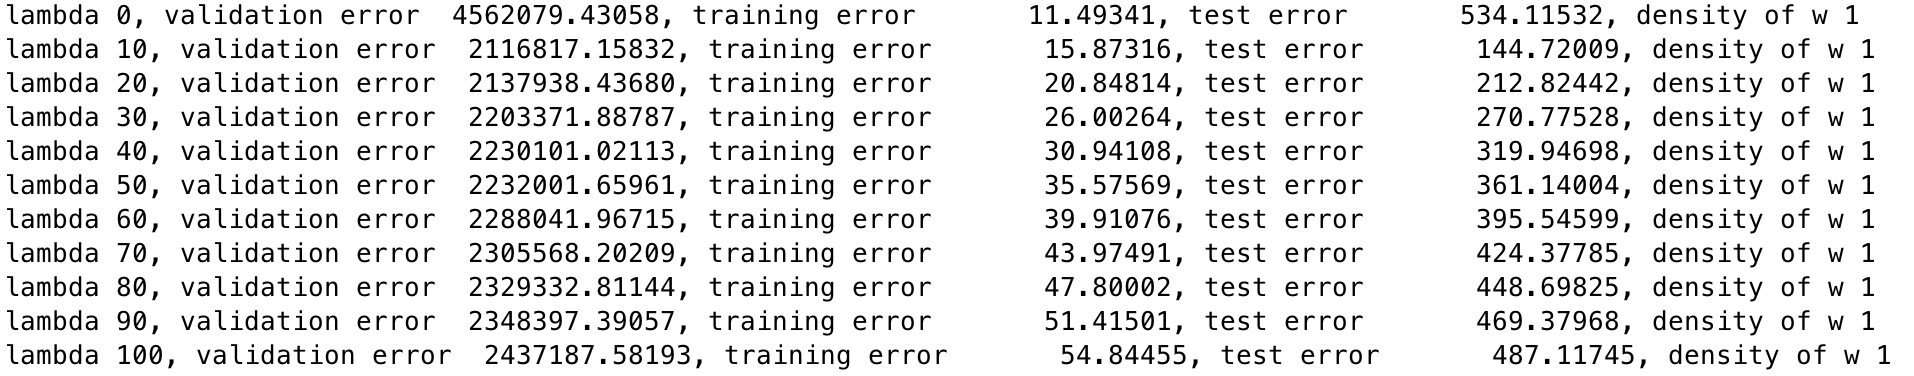
\includegraphics[scale=0.5]{e2q2x}\\
\subsection{question 3}
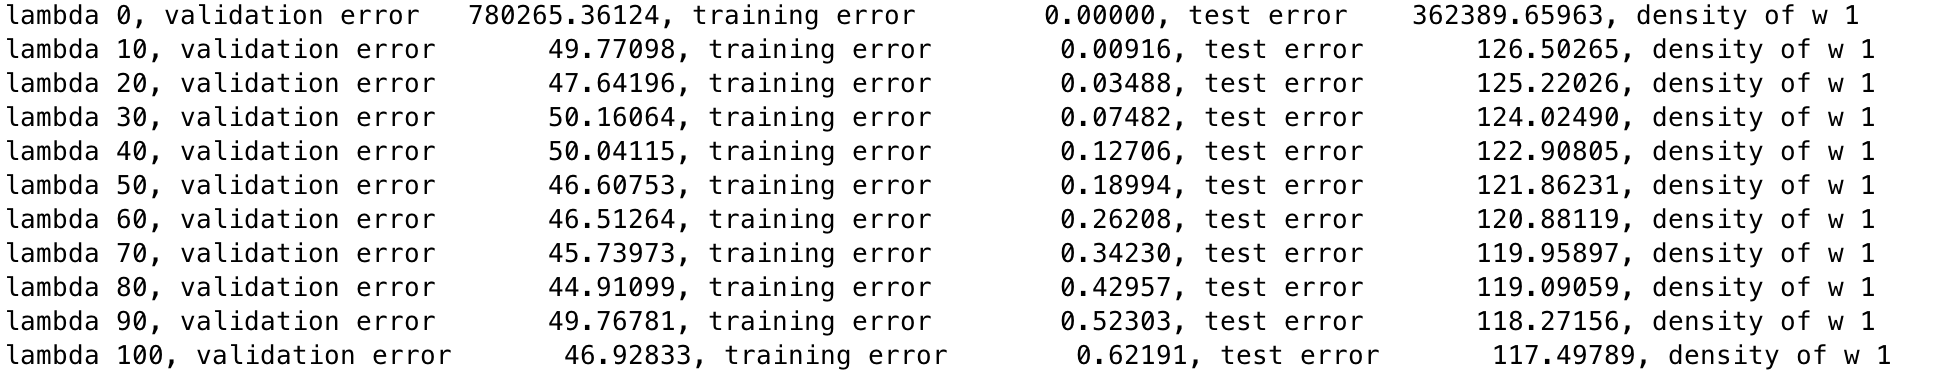
\includegraphics[scale=0.5]{e2q3}\\

\subsection{question 4}
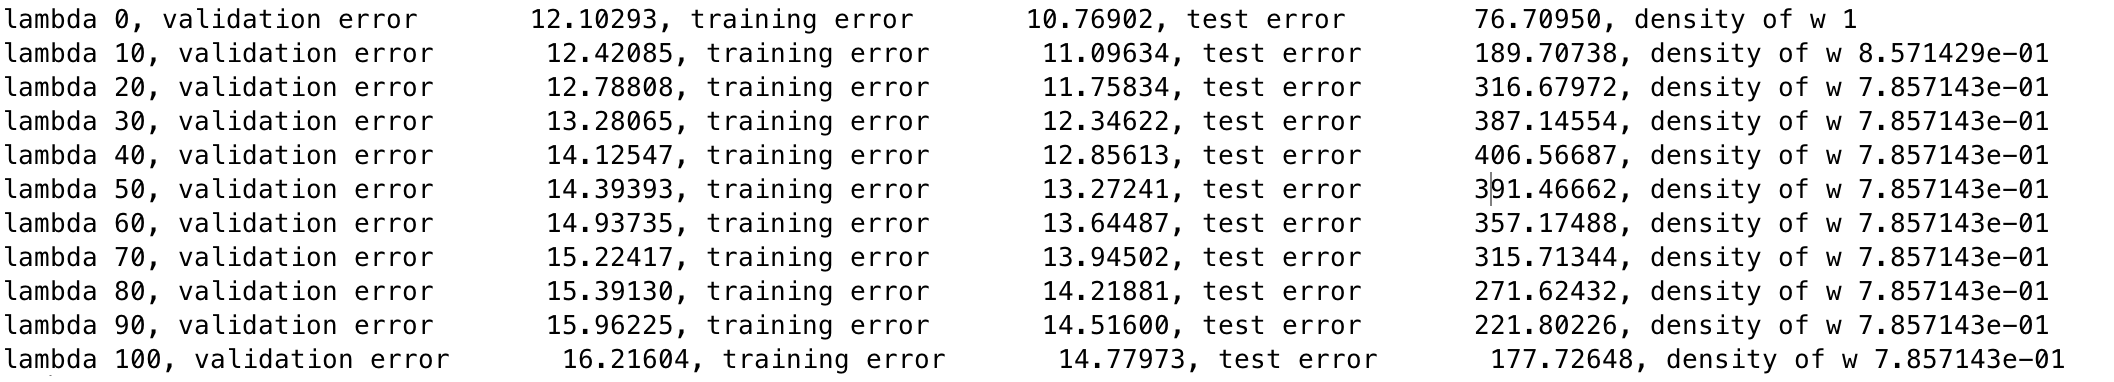
\includegraphics[scale=0.45]{e2q4}\\

\subsection{question 5}
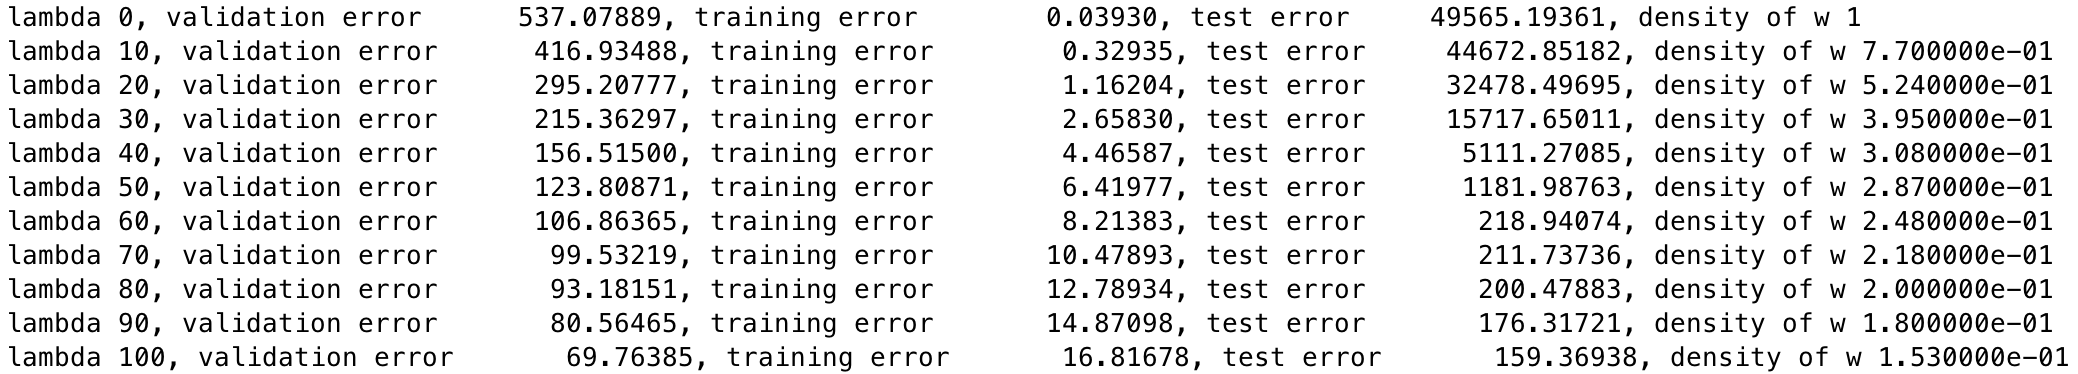
\includegraphics[scale=0.45]{e2q5}\\
Comparing the results with the result from $2.3$, we can see that validation errors in $2.3$ do not differ much, the $lambda$ that produces the smallest validation error does not guarantee the smallest test error. However, in this question, we can see that validation errors for each lambda differ much from each other, the lambda value that produces the smallest validation error also produces the smallest test error. \\
And also, the percentage of $0s$ of w in lasso algorithm is greater than $0\%$, which means in lasso algorithm, not all features are used for prediction, some minor features are ignored. However, in ridge algorithm, the density of $w$ is always 1, which means all features are considered in the process of prediction. 

\end{document}
